\section{Characterization method and results}
\label{Method}
The setup of the noise stage is discussed in sec.~\ref{sec:noisestage}. There exist some differences between the noise stage and the laser stage in the analysis method which discussed in sec.~\ref{sec:laserstage}. 9 MCP-PMTs were tested in testing system. Analysis methods and results are introduced in the following sections.
\subsection{Noise stage}
\label{sec:noisestage}
\begin{figure}[!htbp]
    \centering
    \includegraphics[width=0.5\textwidth,page=1]{figures/method/noisebaseline697_219908_2.pdf}
    \caption{An example of a very large waveform in noise stage. The vertical green line indicates the peak position of pulse candidate. The horizonal blue dash line and horizonal violet dash line are the baseline and amplitude threshold. The rise time and fall time are the width of pink and green rectangle, of which start and end time are interpolated as 10\% and 90\% of rising and falling edges.}
    \label{fig:baseline1}
\end{figure}

The sample window size $T_{\mathrm{wave}}$ is set as \SI{600}{ns}. For \SI{20}{kHz} dark noise rate, the dark noise pulse number obeys Poisson distribution $\pi(\nu=0.012)$ for each wave, which means the probability of 2 or more pulses is about 0.006 times of probability of 1 pulse\footnote{The probability of n dark noise pulse is $P(n)=e^{-\nu}\frac{\nu^n}{n!}$, $P(n=1)=0.012$ and $P(n>1)=7.14\times10^{-5}$}. Considering the pulse width is far short than \SI{600}{ns}, the probability of pulses overlaping with each other is less than 0.006. The maximum peak in time position $t_p$ in each waveform is extracted as the noise pulse candidates as shown in Fig.~\ref{fig:baseline1} and single dark noise pulse events dominate the dataset\footnote{Due to the maximum pulse is calculated, the expected charge distribution is the distribution of $\max_n^N(C_n)$ where $C_n$ is the charge of single PE and $N$ is the number of pulses in a waveform. The bias caused by multipulses is omit.}.


\subsection{Laser stage}
\label{sec:laserstage}

\begin{figure}[!htbp]
    \centering
    \includegraphics[width=0.5\textwidth]{figures/method/triggerwave.pdf}
    \caption{An example of waveform in laser stage. The orange line is the trigger waveform. Two blue horizonal dash line are the upper and lower values of step wave. Green cross point is the interpolation for trigger time. The magnified axes shows the PMT waveform with a signal. Red and green vertical dash line are the time of 10\% of rising edge and pulse peak.}
    \label{fig:triggertime}
\end{figure}

To yield single photon electron (SPE) events, the laser intensity was adjusted to a level only about one out of 20 trigger lead to a signal. The window size $T_{\mathrm{wave}}$ is set to \SI{10400}{ns} and the rising edge of trigger waveform is at about \SI{200}{ns}, which reserve a time interval for pre-pulse analysis. The trigger from the laser system is a step wave, of which the vertical center of rising edge is interpolated to get the trigger time $t_{\mathrm{trig}}$ as shown in Fig.~\ref{fig:triggertime}.

The triggered pulse is mainly centered in the time interval between $[t_{\mathrm{trig}}, 600]$\,ns dependent on the length of cable. The maximum peak is found in the window of $[t_{\mathrm{trig}}, 600]$\,ns to roughly extract the peak position $t_p$. A gaussian function G$(\mu_{t0},\sigma_{t0})$ is unbinned fit to the distribution of peak location of pulses whose peak large than \SI{5}{ADC} for each PMT.% as shown in Fig.~\ref{fig:peaklocation}.

A time interval $[\mu_{t0}-3\sigma_{t0}, \mu_{t0}+3\sigma_{t0}]$ is used for selecting a waveform dataset for each PMT, in which peaks of the triggered wave candidates fall. All the characterizations are calculated with the new time cut which reduces the impact of dark noise.

% \begin{figure}[!htbp]
%     \centering
%     \includegraphics[width=0.4\textwidth]{figures/method/triggerpeakpos.pdf}
%     \caption{Peak location distribution of an example MCP-PMT. A gaussian function is fit to the distribution to acquire an optimized time cut.}%PM
%     \label{fig:peaklocation}
% \end{figure}
\subsection{Baseline}
Due to the offset mentioned in sec.~\ref{sec:setup}, the value of baseline is not zero. A procedure to determine the baseline is developed, which comprised 4 steps as following

1. An interval of the time window $[-t_s,-10]$\,ns ($t_s\in[110,200]$) relative to pulse peak $t_p$ is selected for calculation of baseline. If $t_s < 110$ due to the peak is close to the start of waveform, another interval $[t_p+100,t_p+200]$\,ns is append to the total interval, as shown in Fig.~\ref{fig:baseline1}. Average $\mu_{\mathrm{b0}}$ and standard deviation $\sigma_{\mathrm{b0}}$ of amplitudes in the interval are calculated.

2. An baseline threshold filter $[\mu_{\mathrm{b0}}-\max(\min(5\sigma_{\mathrm{b0}},3),1)]$ is used to remove potential signal and reserve the baseline when $\sigma_{\mathrm{b0}}$ is small.

3. The rest amplitudes are fitted with a gaussian function G$(\mu_{\mathrm{bf}},\sigma_{\mathrm{bf}})$ using unbinned likelihood. $\mu_{\mathrm{bf}}$ and $\sigma_{\mathrm{bf}}$ are accurate at most time. However, when there exists a large wave in the time interval selected in step 1, a bias will be introduced for $\sigma_{\mathrm{bf}}$.

4. Another amplitude filter $[\mu_{\mathrm{bf}}-\min(5\sigma_{\mathrm{bf}},3)]$ is used to reselect the signal area and those areas are padding \SI{10}{ns} at both ends to remove rising edge and falling edge. The rest wave is used to estimate baseline $\mu_b$ and the standard deviation of baseline $\sigma_b$.

\subsection{Peak and charge spectrum}
\label{sec:noisepeak}

The peak $V_p$ of a pulse is the difference between the baseline and minimum of pulse. The charge of a pulse is calculated using integration in a time window $[-15, 75]$\,ns relative to the peak location $t_p$ of the signal as shown in the pink region in Fig.~\ref{fig:triggertime} considering the rise time and fall time distribution, with integration window $T_s$ is \SI{90}{ns}. The equivalent charge $C_{\mathrm{equ}}$ is defined as the summation of the amplitudes in the integration interval. Considering the input impedance is \SI{50}{\Omega}, the true charge of the pulse follows Equ.~\eqref{equ:charge} 
\begin{equation}
    \label{equ:charge}
    C = \frac{C_{\mathrm{equ}}}{50 \Omega}
\end{equation}

\begin{figure}[!htbp]
    \centering
    \includegraphics[width=0.4\textwidth]{figures/method/charge697.pdf}
    \caption{Charge distribution of an example MCP-PMT in noise stage. The vertical green dash line is threshold cut for charge. Origin histogram is the selected entries with peak selection. The red line is the fit Gaussian function for peak. The green line is the fit parabolic function for vally.}
    \label{fig:charge}
\end{figure}

Fig.~\ref{fig:charge} shows the distribution of equaivalent charge of a MCP-PMT in noise stage. The pedestal is a set of waveform with no signal, of which the charge is the summation of baseline and obey Gaussian distribution $G(0, T_s\sigma_b^2)$. The charge of main peak in charge distribution is $\mu_{C_1}$ which is fitted in sec.\ref{sec:noisegain}. To remove the influence of pedestal, pulses of which peaks large than \SI{3}{ADC} and charge large than 0.25$\mu_{C_1}$ are selected. Mean $\mu_{C_{\mathrm{t}}}$ and sample variance $s^2_{C_{\mathrm{t}}}$ of charge of selected pulses are calculated to represent the characteristics of total charge distribution of MCP-PMT. Due to the influence of long tail, the $\mu_{C_{\mathrm{t}}}$ is larger than $\mu_{C_1}$. The physical model and solution of long tail in charge distribution will be discussed in future work.

The charge distribution in laser stage is shown in Fig.~\ref{fig:triggercharge}. Because the statistics is far larger than that of noise stage and the ratio of fluctuation noise is smaller, the P/V ratio is better than noise stage and position of vally is more close to zero. The peak amplitude distribution is shown in Fig.~\ref{fig:triggerpeak} and the bin width of histogram is 1ADC, which shows \SI{3}{ADC} and 0.25$\mu_{C_1}$ threshold are complementary to exclude some noise with small peak height and large charge.

\begin{figure}[!htbp]
    \centering
    \begin{subfigure}[b]{0.4\textwidth}
        \includegraphics[width=\textwidth]{figures/method/triggercharge.pdf}
        \caption{}%PM
        \label{fig:triggercharge}
    \end{subfigure}
    \begin{subfigure}[b]{0.4\textwidth}
        \includegraphics[width=\textwidth]{figures/method/triggerpeak.pdf}
        \caption{}%PM
        \label{fig:triggerpeak}
    \end{subfigure}
    \caption{(a) Charge distribution of an example MCP-PMT in laser stage. (b) Peak distribution of an example MCP-PMT in laser stage. The vertical green dash line is threshold cut for peak. Origin histogram is the selected entries with charge selection.}
\end{figure}

\subsection{Gain and single PE resolution}
\label{sec:noisegain}
There exist a long tail in charge distribution as shown in the histogram with \SI{1}{ADCns} in Fig.~\ref{fig:charge}. To describe the energy resolution of the main peak of the charge distribution, a gaussian function G$(\mu_{C_1},\sigma^2_{C_1})$ is used to fit the binned data via the modified least-square (MLS) method \cite{Cowan1998StatisticalDA} to capture the main peak of charge distribution of the single PE. An interval $[-0.35\mu_{C_1}, 0.35\mu_{C_1}]$ relative to $\mu_{C_1}$ will used to refit the main peak as shown in Fig.~\ref{fig:charge} and Fig.~\ref{fig:triggercharge}. The gain of main peak $G_1$ and gain of total charge $G$ of single PE are calculated as the following equations
\begin{align}
    G_1&=\frac{\mu_{C_1}}{e\times 50\Omega} \\
    G &= \frac{\mu_{C_t}}{e\times 50\Omega}
\end{align}
in which $e$ is the charge of an electron. The main peak resolution and the total charge resolution are defined as
\begin{align}
    \mathrm{Res}_1&=\frac{\sigma_{C_1}}{\mu_{C_1}}\\
    \mathrm{Res}&=\frac{\sqrt{s^2_{C_t}}}{\mu_{C_t}}
\end{align}
Due to the weight of pedestal in noise stage is larger than that of laser stage, the pedestal is more likely to leak into the selected pulses, which has an obvious influence on $\mu_{C_t}$. The variance of resolution and gain in laser stage are better than that in noise stage. Fig.~\ref{fig:totalchargeCompare} shows the 2d distribution of gain and resolution\footnote{The errors of $Res$ and $G$ are estimated using point estimation while errors of $Res$ and $G$ are acquired from ROOT fitting.}. The gain of total charge $G$ is about 2 times of gain of main peak $G_1$ for MCP-PMT, which should be considered in reconstruction. Althogth the resolution of main peak of MCP-PMT is about 0.23, the long tail leads that the resolution of total charge is about 0.69,worse than reference PMT.

\begin{figure}[!htbp]
    \centering
    \includegraphics[width=0.4\textwidth,page=4]{figures/result/compare.pdf}
    \caption{Gain and resolution of total charge and main peak in laser stage. Geen points are reference PMT and red points are MCP-PMT.}
    \label{fig:totalchargeCompare}
\end{figure}
\subsection{Peak-to-valley (P/V) ratio}
A parabolic function is fitted to the vally interval $[-0.15\mu_{C_1}, 0.25\mu_{C_1}]$ relative to the least count bin of histogram between pedestal and SPE peak as shown in Fig.~\ref{fig:charge} and Fig.~\ref{fig:triggercharge}. The local minimum $N_v$ of charge spectrum is calculated as the minima of parabolic function. The $N_p$ is the peak of gaussian function described in sec.~\ref{sec:noisegain}. The peak-to-valley ratio is equal to  
\begin{equation}
    \mathrm{P/V}=\frac{N_p}{N_v}
\end{equation}
The P/V show the ability of discrimination between electronic noise and true signal. The ratio of pedestal also lead to the P/V ratio in laser stage is better than noise stage, as shown in Fig.~\ref{fig:PVCompare}. The mean of P/V ratio of MCP-PMT is $5.79$ in laser stage.
\begin{figure}[!htbp]
    \centering
    \includegraphics[width=0.4\textwidth,page=6]{figures/result/compare.pdf}
    \caption{P/V ratio in noise stage and laser stage} 
    \label{fig:PVCompare}
\end{figure}

\subsection{Rise time, fall time and full width at half maximum (FWHM)}
As shown in Fig.~\ref{fig:baseline1}, $t^{10}_r$, $t^{50}_r$, $t^{90}_r$ are the time of 10\%, 50\% and 90\% amplitude in the rising edge and $t^{10}_f$, $t^{50}_f$, $t^{90}_f$ are the time of 10\%, 50\% and 90\% amplitude in the falling edge which are acquired via interpolation method. The rise time, fall time, and FWHM are calculated as following:
\begin{align}
    t_r &= t^{90}_r - t^{10}_r\\
    t_f &= t^{10}_f - t^{90}_f\\
    \mathrm{FWHM} &= t^{50}_f - t^{50}_r
\end{align}
% \begin{figure}[!htbp]
%     \centering
%     \includegraphics[width=0.4\textwidth]{figures/method/triggerFWHM.pdf}
%     \caption{An example of time characteristics in laser stage.}
%     \label{fig:triggerFWHM}
% \end{figure}
\begin{figure}[!htbp]
    \includegraphics[width=0.4\textwidth,page=7]{figures/result/compare.pdf}
    \caption{Rise time, Fall time, and FWHM}
    \label{fig:RiseCompare}
\end{figure}
Due to some pulse are close to the edge of waveform in noise stage, the rising or falling edge of those pulses are cut by the time window. Therefore only pulses of which peak positions in $[15, T_{\mathrm{wave}}-75]$\,ns are selected in noise stage, while there is the only time interval described in sec.\ref{sec:laserstage} for laser stage.
% Fig.~\ref{fig:triggerFWHM} shows the distribution of rise time, fall time and FWHM of an example MCP-PMT.
The mean and sample variance are calculated in condtion of criteria described in sec.\ref{sec:noisepeak}. The rise time, fall time, and FWHM are consistent between noise stage and laser stage as shown in Fig.~\ref{fig:RiseCompare}. Estimated rise time, fall time and FWHM are .

\subsection{Dark count rate (DCR)}
The dark noise comes from the thermionic electron emitted from photocathode, which generates a pulse signal similar as a photon electron. To discriminate the dark noise with fluctuation of baseline, pulses reach criteria in sec.\ref{sec:noisepeak} are considered as dark noise. The DCR equals to the following equation
\begin{equation}
    \mathrm{DCR/kHz} = \frac{N_{\mathrm{noise}}}{N_{t}}\frac{1}{T_{\mathrm{wave}}/\mathrm{ns}}\times 10^{6}
\end{equation}
in which $N_{\mathrm{noise}}$ is the noise number and $N_{t}$ is the total number of waveforms.

\begin{figure}[!htbp]
    \centering
    \includegraphics[width=0.4\textwidth,page=8]{figures/result/compare.pdf}
    \caption{DCR vs relative PDE}
    \label{fig:DCRCompare}
\end{figure}
The dark count rate and relative PDE of different MCP-PMTs are show in Fig.~\ref{fig:DCRCompare}. The mean DCR is \SI{4.12}{kHz}.
\subsection{Transit time spread (TTS)}
\begin{figure}[!htbp]
    \centering
    \includegraphics[width=0.4\textwidth]{figures/method/triggerTTS.pdf}
    \caption{TT distribution of an example MCP-PMT in laser stage.}
    \label{fig:triggerTTS}
\end{figure}
The TTS is the spread of photo-electron transit time (TT), which represents resolution of timing. The transit time cannot be measured directly, while the trigger time of laser and time of pulse can be measured. A relative transit time $\mathrm{TT}_r$ is defined as the time difference between trigger time $t_{\mathrm{trig}}$ and $t_r^{10}$. The $\mathrm{TT}_r$ distribution is histogramed with \SI{0.5}{ns} bin width. A gaussian fuction G$(\mu_{\mathrm{TT}},\sigma_{\mathrm{TT}}^2)$ is binned fitted to the histogram with interval $[-2,+2]$\,ns relative to the maximum bin using MLS method as shown in Fig.~\ref{fig:triggerTTS}.
% Due to the time precision and voltage precison of FADC are \SI{1}{ns} and \SI{1}{ADC}, the intepolation method TT distribution contains two peak when bin width is smaller than \SI{1}{ns}. 
TTS is defined as
\begin{equation}
    \mathrm{TTS}=2\sqrt{2\ln(2)}\sigma_{\mathrm{TT}}
\end{equation}
% The TTS of different MCP-PMTs are show in Fig.~\ref{fig:TTSCompare}. The mean TTS is \SI{1.78}{ns}.
The mean and standard deviation of measured TTS of 9 PMTs is $\pm$\,ns.
% \begin{figure}[!htbp]
%     \centering
%     \includegraphics[width=0.4\textwidth,page=9]{figures/result/compare.pdf}
%     \caption{TTS versus }
%     \label{fig:TTSCompare}
% \end{figure}
\subsection{Single electron response (SER)}
\begin{figure}
    \centering
    \includegraphics[width=0.4\textwidth]{figures/method/triggerSER.pdf}
    \caption{An fitting result of a pulse.}
    \label{fig:triggerser}
\end{figure}
To get smooth single electron response, the pulses are selected by dedicated cuts:
\begin{itemize}
    \item[1] The amplitude and charge of pulse candidate has to be fulfill the criteria in sec.~\ref{sec:noisegain}.
    \item[2] The FWHM of candidate pulse should exceed \SI{5}{ns} to avoid noise.
    \item[3] To focus on the pulse in the main peak of charge distribution, an upper charge threshold should set. Besides, pulse with small charge is influenced by noise. A charge filter $[0.5C_1, 1000\mathrm{ADCns}]$ is used for reliable results.
\end{itemize}

A gaussian convoluted with an exponential function Equ~\eqref{equ:ser} is used to fit the SER which is shown in Fig.~\ref{fig:triggerser}
\begin{equation}
    \label{equ:ser}
    \mathrm{Gaus}(0,\sigma_t^2)\otimes\theta(t-\mu_t)\frac{1}{\tau}e^{-\frac{t-\mu_t}{\tau}}
\end{equation}
in which $\theta(t)$ is the unit step function, $\mu_t$ is the time offset of pulse, $\sigma_t$ and $\tau_t$ model the shape feature of single electron response. 
\begin{figure}[!htbp]
    \centering
    \includegraphics[width=0.4\textwidth,page=12]{figures/result/compare.pdf}
    \caption{$\tau$ versus $\sigma$}
    \label{fig:sigmaCompare}
\end{figure}

The results of $\tau$ and $\sigma$ are shown in Fig.~\ref{fig:sigmaCompare}. $\tau$ and $\sigma$ of SER is \SI{3.20}{ns} and \SI{1.61}{ns}.

\subsection{Pre-pulse and after-pulse}
The generation of pre-pulses is due to photons hit on the MCP or the first dynode directly rather than the photocathode \cite{JUNOMassTesting}. The amplitude of pre-pulses are smaller than normal signal and appear before the main pulse. This ratio is related to the intensity of light source.
\begin{figure}
    \centering
    \includegraphics[width=0.5\textwidth]{figures/method/triggerAfterpulseSchema.pdf}
    \caption{An example waveform in trigger stage. Green and red vertical dash line are the rising edge of trigger waveform and 10\% of rising edge of main pulse. Dark region is the interval for searching after pulse.}
    \label{fig:afterpulseSchema}
\end{figure}

Afterpulse are generated due to the ionization of gaseous impurities between the cathode and first dynode\footnote{For MCP-PMT, the surface of micro-channel plate is the first dynode.} when photo-electrons go through \cite{Coates_1973}. These ions hit back on the photocathode and generate electrons. \ce{H^+}, \ce{He^+}, \ce{O^+} are the major ions contributing to afterpulse and the relation between time and ions (\ce{^Z_MX}) is $\sqrt{\frac{M}{Z}}$\cite{Coates_1973}. Due to these ions are heavier than electron, the travel time is in the scale of \si{us}\footnote{The velocity of ions is about \SI{1000}{km/s} and size of PMT is about \SI{0.1}{m}, thus the transit time is about \SI{0.1}{us}}. The after pulse is searched in a window \SIrange{100}{10000}{ns} after the main pulse as shown in Fig.~\ref{fig:afterpulseSchema}. The $t$ and $Q$ are calculated as the max peak and integrated in the $[-15,75]$ ns window relative to peak position as shown violet area in Fig.~\ref{fig:afterpulseSchema}
\begin{figure}[!htbp]
    \centering
    \includegraphics[width=0.5\textwidth]{figures/method/triggerAfterpulse1d.pdf}
    \caption{Time distribution of after pulse. The orange and blue histogram are pre-pulse and after-pulse. The green line is the fit result for after pulse. The blank area around the \SI{0}{ns} is the main pulse which is not shown in this figure.}
    \label{fig:afterpulse1d}
\end{figure}
% waveform analysis

Afterpulse is categorized into several kinds. Fig.~\ref{fig:afterpulse1d} indicates 4 typical after-pulse peaks in time around \SI{300}{ns}, \SI{500}{ns}, \SI{1200}{ns} and \SI{1700}{ns}, of which ratio is about $1:\sqrt{2}:\sqrt{16}:\sqrt{32}$. Considering the different mass of ions, these peaks may originate from \ce{H^+}, \ce{He^{2+}}, \ce{O^+}, and \ce{O_2^+} or other unknown ions.

The time distribution and ratio of diferent peaks in afterpulse distribution are parameterized using 4 gaussian functions to model the four peaks as show in Fig.~\ref{fig:afterpulse1d} and the fit equation is as following
\begin{equation}
    N_{\mathrm{trig}}\sum_{i=1}^{4}{A_iG(t_i,\sigma_i^2)}
\end{equation}
in which $A_i$, $t_i$, and $\sigma_i$ are the ratio, time, and width of each peak of after pulse. The fit results are shown in Fig.~\ref{fig:afterpulsePeak} and the ratios of 4 peaks vary greatly for different MCP-PMTs. To be convenient, the mean of ratios and times of peaks are calculated as 1::: and \SI{}{ns}:\SI{}{ns}:\SI{}{ns}:\SI{}{ns}.
\begin{figure}[!htbp]
    \centering
    \includegraphics[width=0.4\textwidth,page=13]{figures/result/compare.pdf}
    \caption{Time and ratio of peaks of after pulse ratio.}
    \label{fig:afterpulsePeak}
\end{figure}
% \begin{figure}[!htbp]
%     \centering
%     \includegraphics[width=0.5\textwidth]{figures/method/triggerAfterpulse2d.pdf}
%     \caption{time and charge distribution of after pulse}
%     \label{fig:afterpulse2d}
% \end{figure}
% Fig.\ref{fig:afterpulse2d} indicates that the after pulse contains some very large signal in the specific peaks, which is different from the distribution of single PE.

The ratio of prepulse $R_{pre}$ is calculated in time interval [-250,-50]\,ns and after pulse $R_{after}$ is calculated in time interval [200,-10000]\,ns. Ratio of pre-pulse and after-pulse is $0.00\pm0.01$ and $0.02\pm0.00$.
\begin{figure}[!htbp]
    \centering
    \includegraphics[width=0.4\textwidth,page=11]{figures/result/compare.pdf}
    \caption{pre-pulse ratio and after-pulse ratio.}
    \label{fig:prepulseCompare}
\end{figure}

\subsection{Relative photon detection efficiency}
The DCR is omit in PDE calculation due to the ratio of dark noise is small. To measure PDE, the intensity of light and light allocation ratio of each channel need to be calibrated. For example, JUNO fixed one reference PMT and other reference PMTs are circulated through all channels \cite{Wonsak_2021}. A new method is designed to reduce the number of reference PMT and combine all test runs to do calibration.

Note $n,j,k$ ($n=0,...,N-1, j=0,...,J-1, k=0,...,K-1$) is the indicator of test run, channel of splitter and PMT. Intensity of light is $I_n$, light allocation ratio is $\alpha_j$ and photon detection efficiency is $\eta_k$. Assume $\alpha_j$s are stable among different test runs. $N_t$ is the total number of waveforms. The photon numbers in each waveform obey Poisson distribution $\pi(p_{njk})$, in which $p_{njk}=I_n\alpha_j\eta_k$. The trigger rate of nth run, kth PMT in jth channel is
\begin{equation}
    \label{equ:pderate}
    R_{njk}=1-e^{-p_{njk}}
\end{equation}
For convenience, 0th PMT is the reference PMT. Note $\alpha_j^0=\frac{\alpha_j}{\alpha_0}$, $\eta_k^0=\frac{\eta_k}{\eta_0}$, $I_n^0=I_n\alpha_0\eta_0$, $i\equiv njk$. $p_{njk}$ can be transfer to Equ~\eqref{equ:pdelograte}
\begin{equation}
    \label{equ:pdelograte}
    \mathrm{log}(p_{njk})=\mathrm{log}(I_0\alpha_0\eta_0)+\mathrm{log}(I_n^0)+\mathrm{log}(\alpha_j^0)+\mathrm{log}(\eta_k^0)
\end{equation}
The relationship between $R_{njk}$ and parameters is
\begin{equation}
    \label{equ:linkfunction}
    R_{njk}=1-e^{-e^{\mathrm{log}(I_0\alpha_0\eta_0)+\mathrm{log}(I_n^0)+\mathrm{log}(\alpha_j^0)+\mathrm{log}(\eta_k^0)}}
\end{equation}
The trigger number $N_{\mathrm{trig}}$ of kth PMT in nth run with jth splitter obey Binomial distribution $B(R_{njk},N_{t_{njk}})$, in which $N_{t_{njk}}$ is total number of waveforms. To fit the parameters, a likelihood is constructed as following
\begin{equation}
    \label{equ:likelihood}
    \mathcal{L}=\prod_{njk}{R_{njk}^{N_{\mathrm{trig}_{njk}}}(1-R_{njk})^{N_{t_{njk}}-N_{\mathrm{trig}_{njk}}}}
\end{equation}

The relationship in Equ.~\eqref{equ:linkfunction} matchs GLM of Binomial exponential family distribution with Cloglog link function\cite{glm}. The GLM is used to maximize the likelihood in Equ.~\eqref{equ:likelihood} and calculate the best value of $\mathrm{log}(\eta_k^0)$ and $\mathrm{log}(\alpha_k^0)$, which is used to calibrate relative photon detection efficiencies and splitter ratios. The results of PDE are show in Fig.~\ref{fig:DCRCompare}. Mean and standard deviation of relative PDE is $1.71\pm$, which is obvious higer than reference PMT.